\section{សំណួរ លំហាត់អនុវត្តន៍ និងកិច្ចការផ្ទះ}
\begin{enumerate}
	\item ចូររកឧទាហរណ៍ទំហំវ៉ិចទ័រ និងទំហំស្កាលែនីមួយៗឲ្យបានប្រាំ។
	\item ចូររកលក្ខណៈខុសគ្នារវាងទំហំវ៉ិចទ័រ និងទំហំស្កាលែ។
	\item តើបម្លាស់ទី និងចម្ងាយចរខុសគ្នាយ៉ាងដូចម្តេច?
	\item ចូរសរសេររូបមន្តល្បឿនមធ្យម និងវ៉ិចទ័រល្បឿនមធ្យម។
	\item តើកុងទ័រម៉ូតូវាស់ចម្ងាយចរ ឬបម្លាស់ទី? ចូរពន្យល់។
	\item តើកុងទ័រម៉ូតូរបស់អ្នកមាននាទីវាស់ល្បឿន ឬវ៉ិចទ័រល្បឿន?
	\item វត្ថុមួយផ្លាស់ទីលើអ័ក្សអាប់ស៊ីសពីចំណុច $x=-1.0cm$ ទៅចំណុច $x_{2}=-4.0cm$។ រកបម្លាស់ទីរបស់វត្ថុនោះ។
	\item រថយន្តមួយត្រូវបានគេបើកបរទៅទិសខាងកើតបានចម្ងាយ $10.0km$ បន្ទាប់មករថយន្ននោះបកត្រឡប់ក្រោយបានចម្ងាយ $4km$។ គណនាចម្ងាយចរ និងបម្លាស់ទីរបស់រថយន្តនេះ។
	\item ចូរបំបែកខ្នាតល្បឿន $54km/h$ ជា $m/s$, $600cm/s$ ជា $km/h$ និង $20m/s$ ជា $km/h$។ 
	\item កីឡាករម្នាក់រត់បានចម្ងាយ $120km$ ដោយប្រើពេល $10.0s$។ តើល្បឿនមធ្យមរបស់កីឡាករនេះស្មើនឹងប៉ុន្មាន?
	\item កីឡាករម្នាក់រត់បានចម្ងាយ $100m$ ដោយប្រើរយៈពេល $10s$។ តើកីឡាករនោះមានល្បឿនប៉ុន្មាន?
	\item រថយន្តមួយចរបានចម្ងាយ $30$ ម៉ាយ ក្នុងរយៈពេល $30$នាទី។ គណនាល្បឿនរបស់រថយន្តគិតជាគីឡូម៉ែត្រក្នុងមួយម៉ោង។
	\item រថយន្នពីរធ្វើចលនាស្មើ។ រថយន្តទី១ ចរបានចម្ងាយ $6km$ ក្នុងរយៈពេល $5mn$ និង រថយន្តទី២ ចរបានចម្ងាយ $90m$ ក្នុងរយៈពេល $3s$។ តើរថយន្តណាមួយមានល្បឿនធំជាង ឬល្បឿនជាង?
	\item តើរថយន្តមួយត្រូវប្រើរយៈពេលប៉ុន្មានម៉ោង ដើម្បីឲ្យរថយន្តនោះចរបានចម្ងាយ $86km$ ក្នុងល្បឿន $8m/s$?
	\item តើយន្តហោះប្រតិកម្មត្រូវមានល្បឿនប៉ុន្មាន $km/h$ ដើម្បីឲ្យល្បឿនរបស់វាស្មើនឹងល្បឿនដំណាលនៃសូរ បើគេដឹងថាល្បឿនដំណាលនៃសូរគឺ $340m/s$។
	\item ក្នុងរង្វិលជុំវិញព្រះអាទិត្យ ផែនដីមានល្បឿន $30km/s$។ គណនាចម្ងាយដែលផែនដីចរបានក្នុងរយៈពេលមួយថ្ងៃមួយយប់ និងក្នុងមួយឆ្មាំគិតជាម៉ែត្រ។
	\item ក្នុងរយៈពេល $\frac{1}{2}mn$ មនុស្សម្នាក់អង្គុយក្នុងរទះភ្ឡើងរាប់បាន $30$ ដងនៃស្នូរដែលកង់រទេះភ្លើងទង្គិចនឹងកន្លែងផ្លូវដែកភ្ជាប់គ្នា។ គណនាល្បឿននៃខ្សែរទេះភ្លើងគិតជា $km/h$ ដោយដឹងថាផ្លូវដែកមួយកំណាត់ៗមានប្រវែង $15m$។
	\item ចម្ងាយរវាងទីក្រុង $A$ និង $B$ ប្រវែង $250km$។ ពីទីក្រុងទាំងពីរ មានរថយន្តពីរចេញដំណើរដំណាលគ្នាដើម្បីជួបគ្នា។ រថយន្តចេញពីទីក្រុង $A$ មានល្បឿន $60km/h$។ រថយន្តចេញពីទីក្រុង $B$ មានល្បឿន $40km/h$។គេសន្មតថា រថយន្តទាំងពីរមានចលនាស្មើ។\\ រករយៈពេលដែលរថយន្តទាំងពីរជួបគ្នាបបន្ទាប់ពីចេញដំណើរ ហើយវាជួបគ្នានៅចម្ងាយប៉ុន្មានពី $A$?
	\item រថយន្តពីរចេញពីភ្នំពេញទៅបាត់ដំបង។ រថយន្តទី១ មានល្បឿន $30km/h$ ចំណែករថយន្តទី២ មានល្បឿន $40km/h$។ រថយន្តទី២ ចេញដំណើរក្រោយរថយន្តទី១ រយៈពេល $10mn$។\\ កំណត់រយៈពេល និងទីកន្លែងដែលរថយន្តទី២ ទៅទាន់ជួបរថយន្តទី១។
	\item កំពង់ផែ $A$ និង $B$ ឋិតនៅចម្ងាយ $46km$ ពីគ្នា។ កំណត់រយៈពេលចាំបាច់សម្រាប់ឲ្យកាណូតមួយចេញពី $A$ ទៅ $B$ រួចពី $B$ ទៅ $A$ វិញ។ ល្បឿនកាណូតក្នុងទឹកនឹងគឺ $13km/h$ និងល្បឿនចរន្តទឹកហូរពី $A$ ទៅ $B$ គឺ $1.5m/s$។
	\item រថយន្តមួយចេញដំណើរពីចំណុច $O$ តម្រង់ទៅទិសខាងលិចដូចបង្ហាញក្នុងរូប។ គណនាសំទុះរបស់វា។
	\begin{figure}[H]
		\centering
		\begin{tikzpicture}
			\begin{scope}
				\draw[->, line width=3pt] (-7,0) --(-8,0);
				\coordinate[label=above:${v=20.0m/s}$] (v1) at (-8,0);
				\coordinate[label=above:${t=10s}$] (t1) at (-4,.7);
				\coordinate[label=above:${v=0}$] (v1) at (3,0);
				\coordinate[label=above:${t=0}$] (t1) at (5,.7);
				\node at (-5,0) {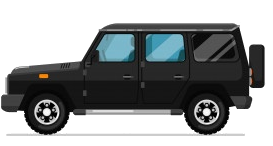
\includegraphics[scale=.4]{car3}};
				\node at (5,0) {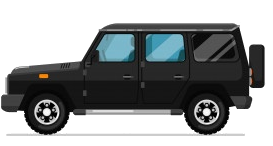
\includegraphics[scale=.4]{car3}};
				\fill[top color=gray, bottom color=gray!30!white] (-8,-1.1) rectangle (8,-.9);
			\end{scope}
		\end{tikzpicture}
	\end{figure}
	\item រថភ្លើងពីរកំពុងផ្លាស់ទីមកជិតគ្នាទៅវិញទៅមកលើគន្លងស្របគ្នា ដែលរថភ្លើងនីមួយៗផ្លាស់ទីដោយល្បឿន $155km/h$ ធៀបនឹងដី។ ប្រសិនបើដំបូងរថភ្លើងទាំងពីរនេះស្ថិតនៅចម្ងាយពីគ្នាប្រវែង $8.5km$។\\ តើរយៈពេលប៉ុន្មាននាទីទើបរថភ្លើងទាំងពីរជួបគ្នា?
	\begin{figure}[H]
		\centering
		\begin{tikzpicture}
		\begin{scope}
		\draw[->, line width=3pt] (-1.5,.5) --(-.5,.5);
		\draw[->, line width=3pt] (1.5,.5) --(.5,.5);
		\draw[->] (.8,2) --(2,2);
		\node at (0,2) {$8.5km$};
		\draw[->] (-.8,2) --(-2,2);
		\coordinate[label=above:${v=155km/h}$] (v1) at (-1,1);
		\coordinate[label=above:${v=155km/h}$] (v2) at (1.8,1);
		\node at (0,0) {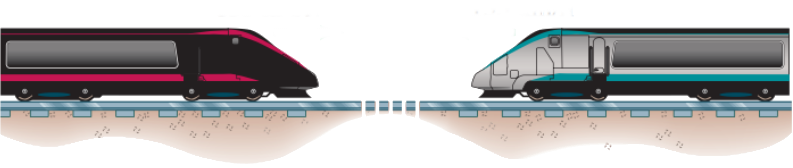
\includegraphics[scale=.5]{train1}};
		\end{scope}
		\end{tikzpicture}
	\end{figure}
%	\item រថយន្តមួយគ្រឿងធ្វើដំណើរដោយល្បឿន $95km/h$ បើកបរតាមពីក្រោយរថភ្លើងមួយដែលមានប្រវែង $1.30km$ ដោយធ្វើដំណើរក្នុងទិសដៅតែមួយនៅលើផ្លូវស្របគ្នា ប្រសិនបើល្បឿនរបស់រថភ្លើង $75km/h$។
%	\begin{enumerate}
%		\item តើរយៈពេលប៉ុន្មានដែលឡានត្រូវប្រើដើម្បីផ្លាស់ទីផុតពីរថភ្លើង។
%		\item ដោយប្រើពេលនេះ តើឡានផ្លាស់ទីបានចម្ងាយប៉ុន្មាន?
%		\item តើនឹងមានអ្វីកើតឡើងប្រសិនបើឡាន និងរថភ្លើងផ្លាស់ទីតាមទិសដៅផ្ទុយគ្នា?
%	\end{enumerate}
%	\begin{figure}[H]
%		\centering
%		\begin{tikzpicture}
%			\begin{scope}
%			\node at (0,0) {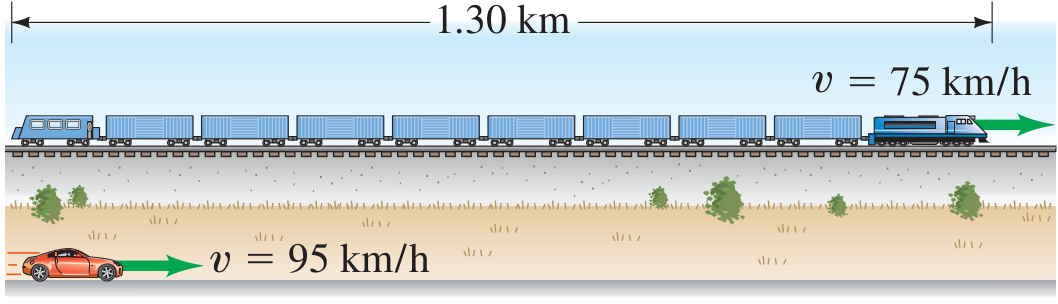
\includegraphics[scale=.40]{car-and-train}};
%			\end{scope}
%		\end{tikzpicture}
%	\end{figure}
	\item ចលនាត្រង់មួយមានសមីការ $x=10+20t-5t^{2}$ ដោយ $x$ គិតជាម៉ែត្រ $\left(m\right)$ និង $t$ គិតជាវិនាទី $\left(s\right)$ ។
	\begin{enumerate}
		\item កំណត់ប្រភេទនៃចលនា និងគណនាសំទុះ។
		\item គណនាល្បឿនខណៈនៅខណៈពេល $t=0$ និង $t=2s$។
		\item តើចល័តស្ថិតនៅទីតាំងណា នៅខណៈដែលល្បឿនរបស់វាមានតម្លៃស្មើសូន្យ។
	\end{enumerate}
	\item អង្គធាតុមួយធ្វើចលនាតាមអ័ក្ស $x'ox$ ដែលមានសមីការ $x=6+2t-t^{2}$ ដែល $x$ គិតជាម៉ែត្រ $\left(m\right)$ និង $t$ គិតជាវិនាទី $\left(s\right)$ ។
	\begin{enumerate}
		\item កំណត់សំទុះ ល្បឿនដើម អាប់ស៊ីសដើម និងប្រភេទចលនា។
		\item គណនាទីតាំង ល្បឿនខណៈ $t=3s$។
	\end{enumerate}
\end{enumerate}